\chapter{Moving Design Optimization}
\label{ch: moving design optimisation}
In the design optimisation of the last chapter, all motions were restrained. Another optimisation is done for moving structures, where the breakwater is able to translate in x-direction and rotate in pitch direction within the xz-plane around its connection point with the floating island. This is done in two design iterations. The first design iteration is discussed in \ref{sec: design iteration 1 moving}. How the optima change while the wave characteristics change is discussed in section \ref{sec: WC2 moving}. \textcolor{red}{The second design iteration is of the moving design optimisation is not yet included in this report.} Finally, the results of the Moving Design Optimisation are discussed in section \ref{sec: discussion moving} and conclusions have been drawn in section \ref{sec: conclusions moving}.\\
\\
% -data took more care, sometimes it was necessary to take a use able part of the data of the simulations. where for the captive optimisation everything was scripted automatically, moving manually\\


\section{Design Iteration 1}
\label{sec: design iteration 1 moving}

The first design iteration's approach is declared in \ref{sec: approach moving H3 DI1}, the correlation between the factors and responses in \ref{fig: correlation DI1 captive} and the design optima are announced in \ref{sec: design optima moving H3 DI1}. 


\subsection{Approach}
\label{sec: approach moving H3 DI1}
The presence of a floating island connected with fenders to the breakwater is imitated by applying a hinge point at the level of the waterline, to the lee-side of the breakwater. Only surge- and pitch motions are allowed. Evidently, a spring force containing surge- and pitch-stiffness is applied in the simulations. The magnitude of the stiffnesses is explained in section \ref{sec: preperation of simulations by Python}.\\
\\
Since again a cubic relation between the factors and responses, a minimum of 94 configurations is required to plot the response surfaces in this order. But, to account for simulations which get unstable and therefore deliver unusable results, a larger design space is used: one with 124 configurations (see appendix \ref{tab: params design iteration 1 moving setup}). The same boundaries as in the captive design optimisation are used, which are repeated in the following table.

\begin{table}[H]
\centering
\scalebox{0.65}{
\begin{tabular}{@{}ccccc@{}}
\toprule
Factor & Name        & Units        & Minimum & Maximum       \\ \midrule
A & T               & m & 2.50   & 13.00   \\
B & W               & m & 10.00  & 150.00   \\
C & front\_fraction & - & 0.01 & 0.99  \\
D & top\_fraction   & - & 0.01 & 0.99  \\
E & radius          & m & 500.00 & 2000.00 \\
F & WL              & m & -6.10  & 4.00     \\ \bottomrule
\end{tabular}
}
\caption{Boundaries Design Space Moving Design Iteration 1}
\label{tab: boundaries DI1 moving}
\end{table}


\subsection{Correlation}
\label{sec: correlation moving H3 DI1}

First thing to notice is that the dependency of most factors on the mean wave drift force is very different in comparison with the captive design optimization. Figure \ref{fig: perturbation R1 DI1 moving H3} shows a complete different trend for the variation of WL (the position of the waterline w.r.t. the breakwater). Although, its optimum lies still beneath the waterline. 
-Note that if two factors are strongly inter-dependent, the trends in the perturbation plots could differ when a value for a certain factor is changed. This effect is shown in figure \ref{fig: perturbation R2 DI1 moving H3} and \ref{fig: perturbation R2 DI1 moving H3 (versie2)}, which is both showing the perturbation of all factors on the wave transmission. Figure \ref{fig: perturbation R2 DI1 moving H3} shows that for breakwaters that have a width of 70 meters, the ideal z-positioning of their body-fixed origin is above the waterline. While figure \ref{fig: perturbation R2 DI1 moving H3 (versie2)} shows that if the width is maximised (W=150), the ideal position is underneath the waterline. In previous design iterations it was observed this level of difference in perturbation plots is quite rare, but in this design iteration it was not.\\
Figure \ref{fig: correlation R1 DI1 moving H3} shows a strong negative correlation on average between the transmission coefficient and the width of the breakwater. Also, a negative correlation between the depth of the breakwater and the wave transmission is observed. The mean wave drift force has a positive correlation with the depth of the breakwater (i.e. a smaller depth leads to a smaller mean wave drift force). 



\begin{figure}[h]
    \centering
    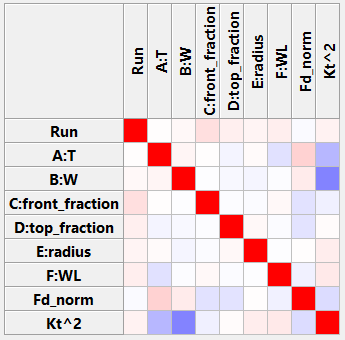
\includegraphics[width=0.3\linewidth]{figures/ComFLOW/Results moving/DI1/H3/correlation_H3.png}
    \caption{Correlation between the factors and responses}
    \label{fig: correlation R1 DI1 moving H3}
\end{figure}


Figure \ref{fig: Fd_norm_VS_top_bw_with_Kt DI1 H3 moving} shows a less visible trend in comparison with the same plot as the captive design optimisation (figure \ref{fig: Fd_norm_VS_top_bw_with_Kt DI1 captive H3}), the points are more scattered. Still several breakwaters experience negative mean wave drift forces, but with the Captive Design Optimisation, almost all breakwaters underneath the waterline experienced negative mean wave drift forces. Figure \ref{fig:  Fd_norm vs Kt DI1 H3 moving} shows configuration 80, 116, 15, 42 and 88 perform good on both having a low mean wave drift force and attenuating much of the wave energy.

\begin{figure}[h]
    \centering
    \begin{subfigure}[b]{0.49\textwidth}
        \centering
        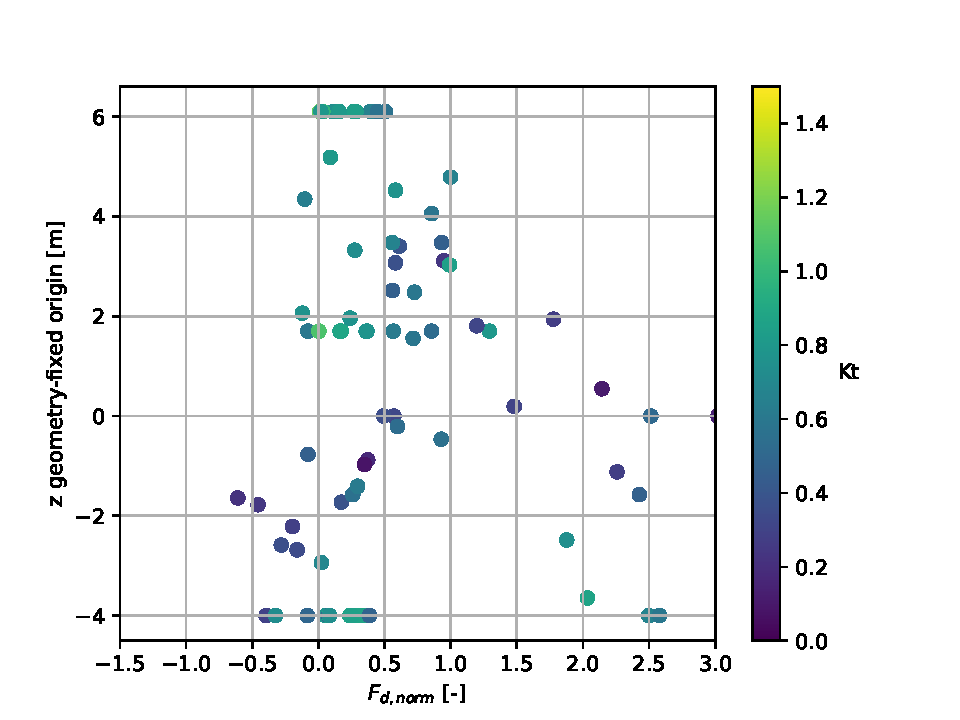
\includegraphics[width=\linewidth]{figures/ComFLOW/Results moving/DI1/H3/Fd_norm_VS_top_bw_with_Kt.pdf}
        \caption[]%
        {{\small }}    
        \label{fig: Fd_norm_VS_top_bw_with_Kt DI1 H3 moving}
    \end{subfigure}
    \hfill
    \begin{subfigure}[b]{0.49\textwidth}  
        \centering 
        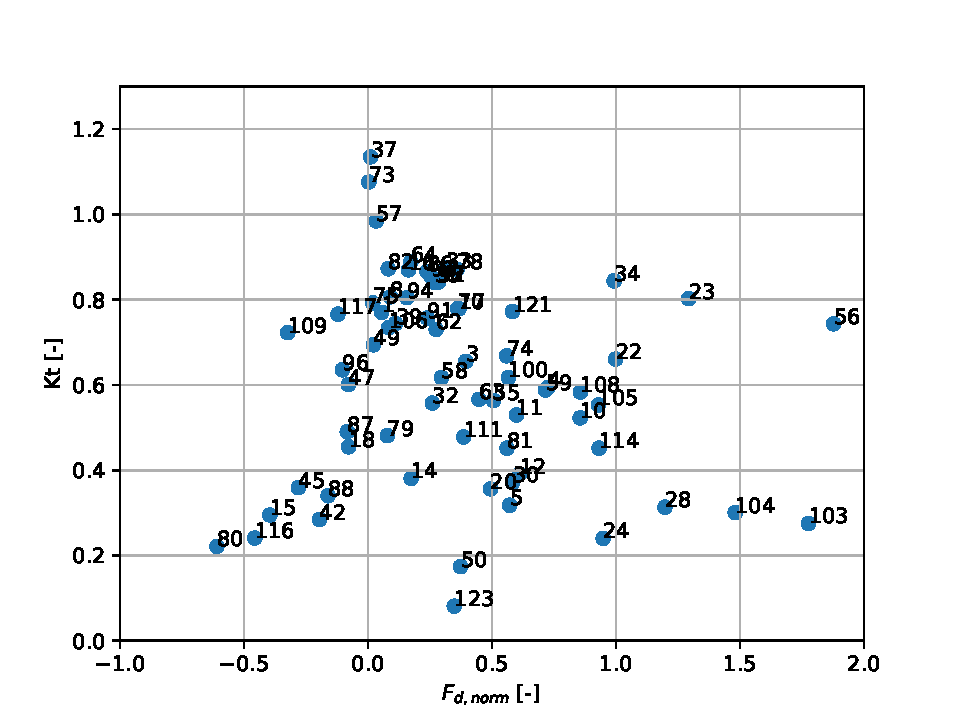
\includegraphics[width=\linewidth]{figures/ComFLOW/Results moving/DI1/H3/Fd_norm_VS_Kt.pdf}
        \caption[]%
        {{\small }}    
        \label{fig:  Fd_norm vs Kt DI1 H3 moving}
    \end{subfigure}
    
    \caption{Results ComFLOW design space breakwaters}
    \label{fig: }
\end{figure}



%\subsection{Response Surfaces}

\subsection{Design Optima}
\label{sec: design optima moving H3 DI1}




%%%%%%%%%%%%%%%%%%%%%%%%%%%%%%%%%%%%%%%%%%%%%%%%%%%%%%%%%%%%%%%%%%%%%%%%%%%%%%%%%%%%
\subsubsection{Based on minimal mean wave drift force}

Various optima with as goal minimising the mean wave drift force and vary a lot compared with the \acrlong{cdo}. The width $W$ of most optima is relatively large and also the depth did not converge to the lower boundary. Also, the first two optima do have a sloping beach, but the rest have a large front\_fraction. They are placed almost four meters beneath the water level. 

\begin{table}[H]
\centering
\scalebox{0.65}{
\begin{tabular}{@{}ccccccccccc@{}}
\toprule
configuration & T        & W        & front\_fraction & top\_fraction & radius   & WL & $F_{d,norm,DoE}$ & $K_{t,DoE}^2$  & $F_{d,norm,ComFLOW}$  & $K_{t,ComFLOW}^2$      \\ \midrule
1  & 3.00 & 76.68  & 0.02 & 0.63 & 1331.63 & 3.85 & -1.79 & 0.28 &  &  \\
2  & 2.88 & 107.77 & 0.01 & 0.77 & 1980.29 & 3.55 & -1.67 & 0.23 &  &  \\
3  & 8.59 & 38.82  & 0.95 & 0.99 & 1465.29 & 4.00 & -1.52 & 0.39 &  0.16 & 0.38 \\
4  & 3.28 & 85.79  & 0.97 & 0.43 & 905.24  & 3.78 & -1.60 & 0.28 &  &  \\
5  & 8.53 & 11.46  & 0.95 & 0.03 & 1261.90 & 3.87 & -1.75 & 0.70 &  &  \\
6  & 3.93 & 53.98  & 0.97 & 0.24 & 1531.32 & 3.79 & -1.51 & 0.31 &  &  \\
7  & 2.55 & 90.71  & 0.98 & 0.73 & 1199.47 & 3.51 & -1.61 & 0.26 &  &  \\
8  & 2.62 & 144.71 & 0.99 & 0.90 & 527.11  & 3.96 & -1.58 & 0.24 &  &  \\
9  & 2.64 & 137.95 & 0.99 & 0.38 & 564.07  & 0.77 & -1.55 & 0.18 &  &  \\
10 & 3.33 & 92.60  & 0.97 & 0.60 & 1652.94 & 3.56 & -1.55 & 0.27 &  &  \\ \bottomrule
\end{tabular}
}
\caption{Parameters optimal breakwaters based on minimal mean wave drift force}
\label{tab: params design iteration 1 moving br 1to10 mean wave drift force}
\end{table}


\begin{figure}[h]
    \centering
    \begin{subfigure}[b]{0.49\textwidth}
        \centering
        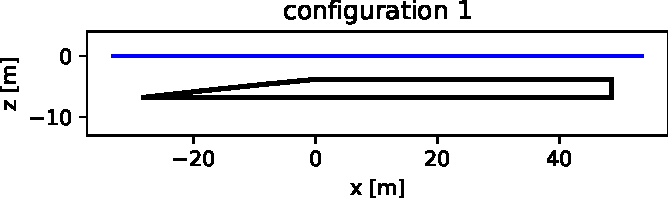
\includegraphics[width=\textwidth]{figures/ComFLOW/Breakwater Geometries/DI1 moving/optima_Fd/breakwater_geometry1.pdf}
        \caption[]%
        {{\small}}    
        \label{fig: opt breakwater 1 moving fd}
    \end{subfigure}
    \hfill
    \begin{subfigure}[b]{0.49\textwidth}  
        \centering 
        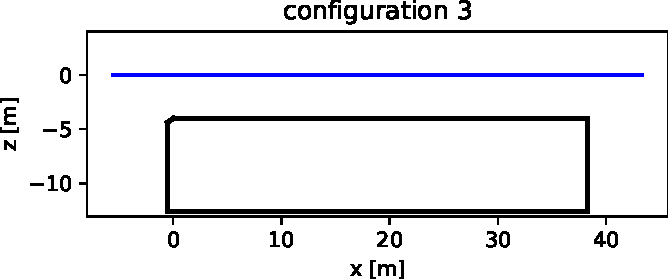
\includegraphics[width=\textwidth]{figures/ComFLOW/Breakwater Geometries/DI1 moving/optima_Fd/breakwater_geometry3.pdf}
        \caption[]%
        {{\small}}    
        \label{fig: opt breakwater 3 moving fd}
    \end{subfigure}
    
    \caption{The two most optimal breakwaters based on the mean wave drift force}
    \label{fig: two most optimal breakwaters moving fd}
\end{figure}





%%%%%%%%%%%%%%%%%%%%%%%%%%%%%%%%%%%%%%%%%%%%%%%%%%%%%%%%%%%%%%%%%%%%%%%%%%%%%%%%%%%%
\subsubsection{Based on minimal transmission coefficient}

In order to minimise the transmission coefficient of the breakwaters, different optima were found as well. Structures with a large $W$ underneath the water surface and structures with a large depth and a relatively small $W$ placed higher, crossing the water surface.  

\begin{table}[H]
\centering
\scalebox{0.65}{
\begin{tabular}{@{}ccccccccccc@{}}
\toprule
configuration & T        & W        & front\_fraction & top\_fraction & radius   & WL & $F_{d,norm,DoE}$ & $K_{t,DoE}^2$  & $F_{d,norm,ComFLOW}$  & $K_{t,ComFLOW}^2$      \\ \midrule
1  & 10.33 & 65.81  & 0.91 & 0.33 & 1756.14 & -1.85 & 1.59  & -0.07 &  0.28 & 0.14 \\
2  & 5.21  & 146.91 & 0.02 & 0.90 & 1909.84 & 3.56  & 1.61  & -0.01 &  &  \\
3  & 7.99  & 53.92  & 0.97 & 0.37 & 980.90  & -2.61 & 0.59  & -0.01 &  &  \\
4  & 10.92 & 58.04  & 0.75 & 0.94 & 1411.90 & -1.22 & 1.94  & -0.05 &  &  \\
5  & 8.35  & 49.86  & 0.80 & 0.08 & 1197.96 & -1.27 & 1.12  & -0.01 &  &  \\
6  & 6.75  & 148.56 & 0.96 & 0.56 & 957.66  & 3.46  & -0.17 & -0.01 &  &  \\
7  & 8.66  & 71.63  & 0.96 & 0.02 & 1983.91 & -2.95 & 0.55  & -0.01 &  &  \\
8  & 8.74  & 47.08  & 0.02 & 0.99 & 698.74  & -1.31 & 0.76  & 0.00  &  &  \\
9  & 12.41 & 146.74 & 0.91 & 0.98 & 513.68  & -0.13 & 3.04  & 0.00  &  &  \\
10 & 8.83  & 148.10 & 0.75 & 0.80 & 1407.54 & 3.95  & 2.59  & -0.06 &  &  \\ \bottomrule
\end{tabular}
}
\caption{Parameters optimal breakwaters based on minimal transmission coefficient}
\label{tab: params design iteration 1 moving br 1to10 transmission}
\end{table}

\begin{figure}[h]
    \centering
    \begin{subfigure}[b]{0.49\textwidth}
        \centering
        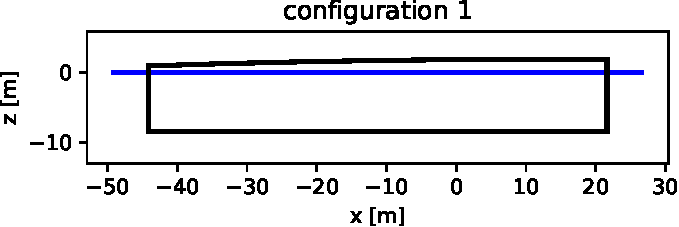
\includegraphics[width=\textwidth]{figures/ComFLOW/Breakwater Geometries/DI1 moving/optima_Kt/breakwater_geometry1.pdf}
        \caption[]%
        {{\small}}    
        \label{fig: opt breakwater 1 moving kt}
    \end{subfigure}
    \hfill
    \begin{subfigure}[b]{0.49\textwidth}  
        \centering 
        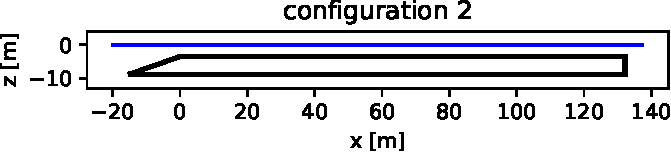
\includegraphics[width=\textwidth]{figures/ComFLOW/Breakwater Geometries/DI1 moving/optima_Kt/breakwater_geometry2.pdf}
        \caption[]%
        {{\small}}    
        \label{fig: opt breakwater 2 moving kt}
    \end{subfigure}
    
    \caption{The two most optimal breakwaters based on the transmission coefficient}
    \label{fig: two most optimal breakwaters moving kt}
\end{figure}


% \subsection{Discussion}
% -trend of negative mean wave drift forces still there, but less visible-->maybe because due to pressure difference the breakwater moves in x-direction to counteract, therefore the mean pressure difference between fore and aft of the breakwater less present and therefore not so much negative mean wave drift force.



% \subsection{Conclusion}


